\section{Introduction}

\label{sec:intro}
Large-scale vision-language pre-training has attracted wide research interests in recent years~\cite{uniter, albef, clip, uniperceiver}. Different from training independent models for each specific task, pre-trained models take the analogy of human biological intelligence system, trying to perceive the world from various data modalities and handle comprehensive tasks. Specifically, it aims to provide a unified inference paradigm that simultaneously learns representations for multi-modal data and can easily transfer to a variety of downstream tasks. Benefiting from the accessibility of massive image-text pairs from the web, the vision-language pre-training can leverage a broader source of supervision, and effectively improves the model's generalization power.

Early attempts on vision-language pre-training mainly focus on detecting objects in the images and aligning the corresponding word tokens with object regions~\cite{uniter,oscar,lxmert}. Though effective, the entanglement with the concept of objects, and the additional resources for pre-trained object detectors impose restrictions on real-world applications. One of the pioneer works, CLIP~\cite{clip}, extends the scale of the pre-training dataset to 400 million image-text pairs, and learns representations by directly matching raw text with the corresponding image. Through a contrastive-based training scheme, CLIP learns visual concepts under a large vocabulary which significantly improves the model performances on various downstream tasks. Taking inspiration from CLIP, the following researches further extend the work from several perspectives, including data modality~\cite{uniperceiver}, downstream tasks~\cite{ofa}, and training data efficiency~\cite{clipnoise, cliplite}.

\begin{figure}[t]
  \centering
  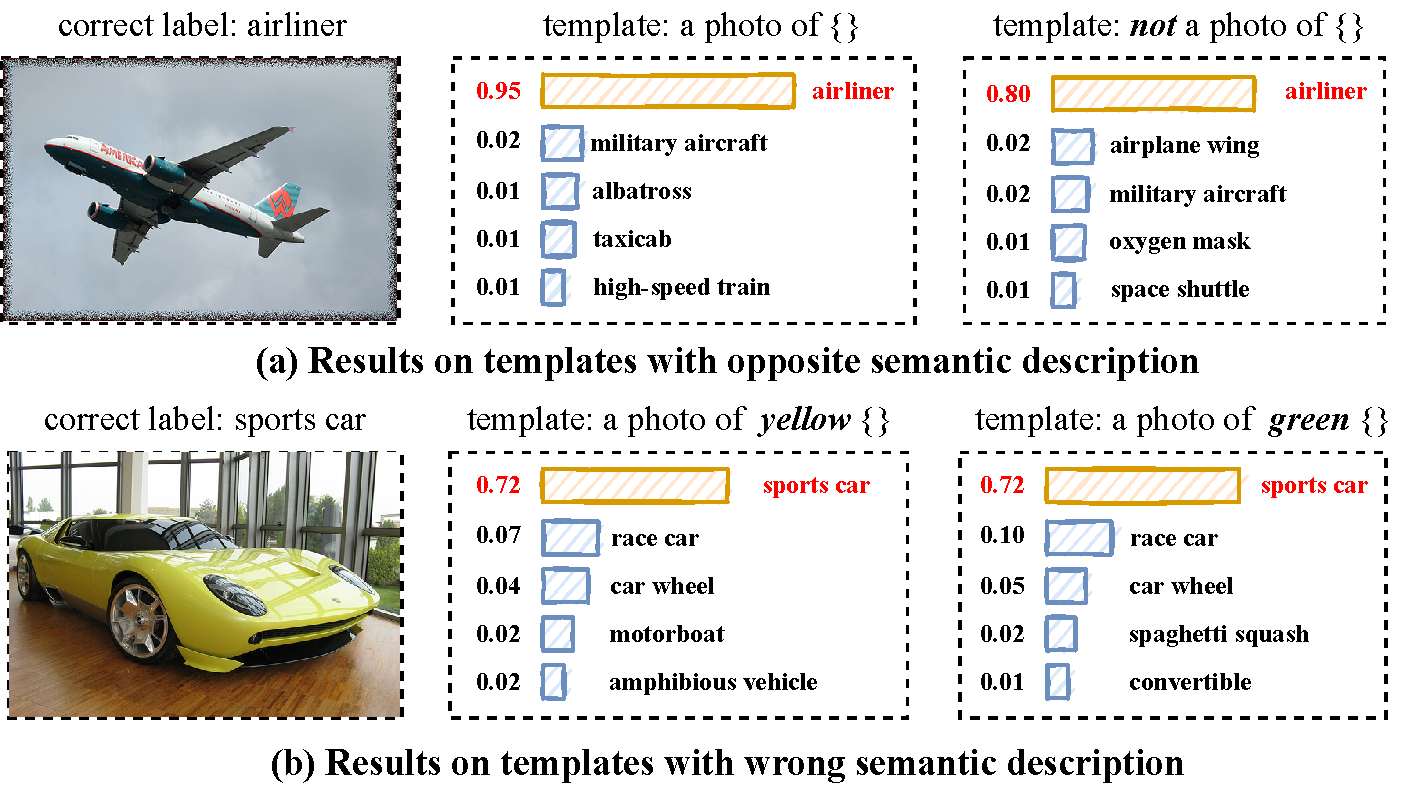
\includegraphics[width=1.0\linewidth]{1_3.pdf}
  \vskip -0.1in
  \caption{CLIP fails to accurately capture some fine-grained semantic information. When given opposite semantic descriptions, \textit{e.g.,} adding 'not' in the template or describing an image with wrong color, CLIP tends to give similar distribution as the correct counterpart. Best view in color.}
\vskip -0.1in
\label{fig1}
\end{figure}

Although showing promising results, the current pre-training frameworks also suffer from limitations. Specifically, the data pairs for pre-training are organized in the simplest manner, where only the descriptions of \textit{matched} and \textit{unmatched} are used to represent the relation between a given image and text pair. This usually leads to a degenerated scenario, where the model tends to rely on the co-occurrence of inputs instead of their semantic meanings. 
% As a showcase, we consider a toy example by evaluating the zero-shot transfer performance of CLIP on the ImageNet dataset~\cite{imagenet} with the templates 'a photo of a \{\}' and 'not a photo of a \{\}', and show the results in Fig.~\ref{fig1}.
We give a toy example in Fig.~\ref{fig1} by evaluating the zero-shot transfer performance of CLIP on the ImageNet dataset~\cite{imagenet} with the templates 'a photo of a \{\}' and 'not a photo of a \{\}'. It is shown that the distributions of CLIP outputs under two templates are quite similar, suggesting that the current model fails to understand the semantic meaning of word tokens. As a result, the transferability of the model is restricted, and tends to show worse performances on tasks that require reasoning ability, \textit{e.g.,} visual question answering.

% Second, current vision-language pre-training approaches face a dilemma on the scope of image perceiving. On one hand, detector-based models recognize fin-grained regions in an image, while under the restriction of detecting real objects. On the other hand, models like CLIP view the whole image as a single input, making it difficult to deal with more abstract and systematic tasks. This contradiction leaves the model with incomprehensive perceptions for image inputs.

% Second, due to the demand on large-scale image-text pairs, the pre-training procedure is greatly prolonged and computation expensive. The hundreds or even thousands of GPU days training prohibits frequent 


To address the limitation of pre-trained models on semantic perceiving, we resort to the technique of knowledge graph, which has been widely studied in the field of natural language processing~\cite{kgreason,kgembed}. Knowledge graph (KG) is a large-scale semantic network that comprises entities as nodes and semantic relations as edges. Through organizing data in a graph structure, knowledge graphs provide rich information on describing the relations between entities and enable a reasoning process through the whole graph. These advantages over regular-structured data are favorable on various tasks including question-answering~\cite{kgqa, kgqa2}, relation prediction~\cite{kgrel2,kgrel} and knowledge reasoning~\cite{kgkreason, kgkreason2}. In recent years, knowledge graph has also been investigated in the field of computer vision, \textit{e.g.}, scene graph~\cite{sggen}, and the integration of both language and image~\cite{visualsem}. This bridges the gap between different modalities in the knowledge graph, which inspires us to explore a new knowledge-based pre-training framework, and inject semantic information into simple image-text pairs.

In this paper, we propose a novel vision-language pre-training approach, dubbed \textit{Knowledge-CLIP}, by constructing a knowledge augmented pre-training framework based on the widely used CLIP models. As illustrated in Fig.~\ref{fig3}, we follow the structure of CLIP, and use two Transformer-based models as image and text encoders respectively. These two encoders take entities and relations in the knowledge graph as input and extract raw features for both entities and relations. Notably, entities can be in the form of image/text, while the relations are constantly described by language tokens. Then, a multi-modal Transformer encoder is adopted to fuse the entity features conditioned on their relations. In this way, the pre-trained model is pushed to concentrate on understanding semantic relations between visual and word concepts, thereby establishing strong semantic connections between vision and language modalities. 

To additionally improve the training efficiency and avoid the massive computation cost in the pre-training procedure, we adopt a simple continuous learning strategy by training our model based on the pre-trained weights of CLIP. This provides a possibility of efficiently promoting the model performance of CLIP with low training resources. 

We train our model on three knowledge graph datasets, namely Visual-Genome~\cite{vgdata} (scene graph), ConceptNet~\cite{conceptnet} (language-based graph), and VisualSem~\cite{visualsem} (multi-modal graph), and also adopt part of datasets from CLIP to avoid the model forgetting problem. With the knowledge-enhanced pre-training, Knowledge-CLIP achieves consistent improvements over the original CLIP models on various vision and language downstream tasks. 
% Our model can also transfer to several graph-based tasks, including link prediction and entity classification, and achieve competitive results.